\section{Evaluation}
\labsection{evaluation}

This section presents a performance study of our \SPSER transactional memory described in \refsection{stm}.
To conduct this evaluation we implemented and integrated our algorithm inside \textsc{TinySTM}~\cite{FelberFMR10}, a state-of-the-art software transactional memory implementation.
Our modifications account for approximatively 500 SLOC.
We run \refalg{stm} in disjoint-access parallel mode.
As explained in \refsection{stm:discussion}, in this variation the clocks of the processes are not accessed.
A detailed evaluation of the other variations of \refalg{stm} is left for future work.

The experiments are conducted on an AMD Opteron48, a 48-cores machine with 256 GB of RAM. 
This machine has 4 dodeca-core AMD Opteron 6172, and 8 NUMA nodes.
To evaluate the performance of our implementation on this multi-core platform, we use the test suite included with \textsc{TinySTM}.
This test suite is composed of several TM applications with different transaction patterns.
The reminder of this section briefly describes the benchmarks and discuss our results.
As a matter of a comparison, we also present the results achieved with the default \textsc{TinySTM} distribution, (v1.0.5).
 
\subsection{A bank application}
\labsection{evaluation:bank}

The bank benchmark consists in simulating transfers between bank accounts.
A transaction updates two accounts, transferring some random amount of money from one account to another.
A thread executing this benchmark performs transfers in closed-loop.
Each thread is bound to some \emph{branch} of the bank, and accounts are spread evenly across the branches.
A \emph{locality} parameter allows to tune the accounts accessed by a thread to do a transfer.
This parameter serves to adjust the probability that a thread executes consecutive operations on the same data.
More specifically, when locality is set to the value $\rho$, a thread executes a transfer in its branch with probability $\rho$ and between two random accounts with probability $(1-\rho)$.
When $\rho=1$, this workload is fully parallel.

\reffigure{bank} presents the experimental results for the bank benchmark.
In \reffigure{bank:base}, we execute a base scenario with 10k bank accounts, and a locality of 0.8.
We measure the number of transfers performed by varying the number of threads in the application.
In this figure, we observe that the performance obtained with \textsc{TinySTM} merely improves as the number of thread increases: 48 threads achieve $2.8$ million transactions per second (MTPS), scaling-up from $2.2$ MTPS with a single thread.
Our implementation performs better: with 48 threads \refalg{stm} executes around 68 MTPS, executing $\times 31$ more operations than with one thread.

To understand the impact of data locality on performance, we vary this parameter for a fixed number of threads.
\reffigure{bank:speedup} presents the speedup obtained when varying locality from $0$, i.e., all the accounts are chosen at random, up to $1$, where they are all chosen in the local branch.
In this experiment, we fix the number of threads to $48$, \emph{i.e.} the maximum number of cores available on our test machine.
As shown in ~\reffigure{bank:speedup}, our TM implementation leverages the presence of data locality in the bank application.
This is expected, since we use the disjoint-access parallel (DAP) variation of \refalg{stm}.
When locality increases, the contention in the application decreases.
As a consequence of DAP, each thread works on independent data, thus improving performance.

\begin{figure}[!t]
  \centering
  \subfigure[Base scenario -- locality set to $0.8$]{
    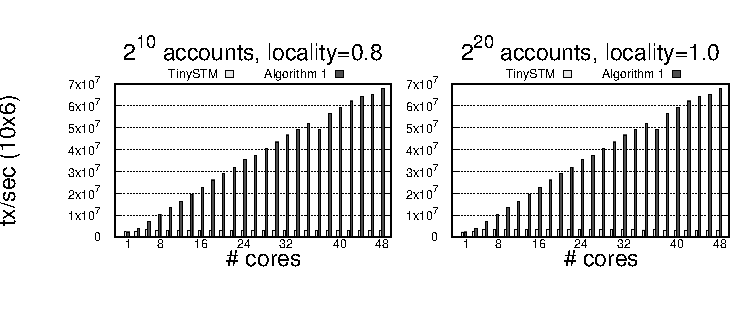
\includegraphics[scale = 0.8]{results/intset/bank.pdf}
    \labfigure{bank:base}
  }
  \subfigure[Varying locality -- using $48$ threads]{
    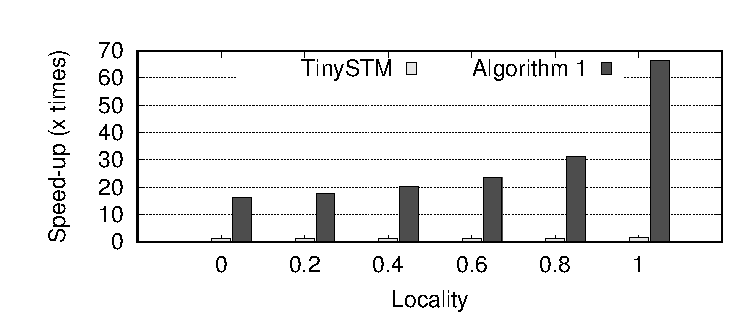
\includegraphics[scale = 0.8]{results/bank-speedup/bank-speedup.pdf}
    \labfigure{bank:speedup}
  }
  \caption{
    \labfigure{bank}
    Bank benchmark with fixed locality (a) and increasing locality values (b).
  }
\end{figure}

\subsection{Linked-list}
\labsection{evaluation:ll}

The linked-list benchmark consists in concurrently modifying a sorted linked-list of integers. 
Each thread randomly adds or removes an integer from the list. 
We run this benchmark for a range of $512$ values, \emph{i.e.} a thread randomly selects a value between $-255$ and $+256$ before doing an insertion/removal.
The linked list is initialized to contain $256$ integers.
We report our results in \reffigure{llrb}~(left).

We observe that \textsc{TinySTM} outperforms our implementation in the linked-list benchmark.
This is due to the fact that, without proper clock synchronization, transactions tend to re-validate their reads frequently over their execution paths.
In this scenario of high contention, it is (as expected) preferable to rely on a frequent synchronization mechanism such as the global clock used in \textsc{TinySTM}.
To alleviate this issue, one could adjust dynamically the clocks used in \refalg{stm} accordingly to contention. 
Such a strategy could rely on a global lock, similarly to the mechanism used to avoid that long transactions abort.
We left the implementation of this optimization for future work

\begin{figure}[!t]
  \centering
  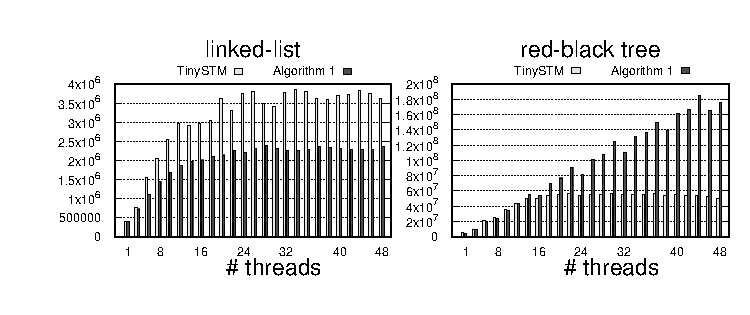
\includegraphics[scale = 1.0]{results/intset/ll-rb.pdf}
  \caption{Linked-list (left) and Red-Black tree (right) benchmarks. Y-axis: transactions/sec. \labfigure{llrb}}
\end{figure}

\subsection{Red-Black Tree}
\labsection{evaluation:rb}

The red-black tree benchmark is similar to the linked-list benchmark except that the values are stored in a self-balancing binary search tree. 
We run this benchmark with a range of $10^7$ values, and a binary tree initialized with $10^5$ values.
\reffigure{llrb}~(right) reports our results.

When using the original \textsc{TinySTM} design, the performance of the application improves linearly up to 12 threads. 
It then stalls to approximately 50 MTPS due to contention on the global clock.
In this benchmark, the likelihood of having two concurrent conflicting transactions is very low.
Leveraging this workload property, our implementation of \refalg{stm}, scales the application linearly with the number of threads.
\refalg{stm} achieves 176 MTPS with 48 threads, improving performance by a $\times 36$ factor over a single threaded execution.


